% Online (supplemental) appendix: submitted as a separate PDF. Not typeset by the AER.
% The main paper must be self-contained without it.
\documentclass[12pt]{article}
\usepackage[margin=1in]{geometry}
\usepackage[T1]{fontenc}
\IfFileExists{lmodern.sty}{\usepackage{lmodern}}{}
\usepackage{amsmath,graphicx,booktabs,xcolor,setspace}
\usepackage[round,authoryear]{natbib}
\usepackage{hyperref}
\graphicspath{{../figures/}}
\onehalfspacing
\newcommand{\todo}[1]{{\color{red!70!black}\small\textsf{[TODO: #1]}}}
\newcommand{\ES}{\textsc{es}}\newcommand{\NQ}{\textsc{nq}}\newcommand{\ZN}{\textsc{zn}}\newcommand{\YM}{\textsc{ym}}
\renewcommand{\thesection}{OA.\arabic{section}}
\renewcommand{\thetable}{OA.\arabic{table}}
\renewcommand{\thefigure}{OA.\arabic{figure}}

\title{Online Appendix to\\ ``Surprises, Shapes or Machines? Forecasting the Market's Response to Macroeconomic Releases with Dynamic Time Warping (DTW)''}
\author{Benjamin Steel, Jack Duncan, Aaryen Mehta, Reza Zamani and Hoshea Zeng}
\date{}
\begin{document}
\maketitle

\section{Release families traded by market}
Table~\ref{oa:families} lists the release families admitted by the impact screen in at least one
year from 2018 to 2026 (rank in the screen at the start of 2026 in parentheses). CPI is always
traded.

\begin{table}[htbp]
  \centering\small
  \caption{Release families admitted by the impact screen (top ten in at least one year, 2018--2026).}
  \label{oa:families}
  \footnotesize\begin{tabular}{p{0.22\linewidth}p{0.22\linewidth}p{0.22\linewidth}p{0.22\linewidth}}
    \toprule
    \ES & \NQ & \ZN & \YM \\
    \midrule
    CPI (1), Employment Report (2), Fed interest on reserves (3), FOMC decision (4), ISM
    Manufacturing (5), U.\ of Michigan (6), ISM Services (7), ISM Services Prices Paid (8), JOLTS (9),
    Case--Shiller NSA (10), Retail Sales, S\&P Global Manufacturing PMI, GDP, Trade Balance,
    Philadelphia Fed, IBD/TIPP
    &
    CPI (1), Employment Report (2), Fed interest on reserves (3), FOMC decision (4), Dallas Fed (5),
    U.\ of Michigan (6), ISM Manufacturing (7), ISM Services (8), ISM Services Prices Paid (9), PPI
    (10), ISM Milwaukee, Retail Sales, S\&P Global PMIs, Conference Board, Trade Balance, GDP
    &
    ISM Services Prices Paid (1), Employment Report (2), FOMC decision (3), CPI (4), ISM New Orders
    (5), ISM Manufacturing (6), ISM Services (7), Fed interest on reserves (8), S\&P Global PMIs (9,
    10), Retail Sales, Factory Orders, FHFA, U.\ of Michigan, Trade Balance
    &
    Employment Report (1), Fed interest on reserves (2), CPI (3), FOMC decision (4), ISM
    Manufacturing (5), Retail Sales (6), ISM Services (7), JOLTS (8), PPI (9), Trade Balance (10),
    Business Inventories, U.\ of Michigan, GDP, Wholesale Inventories, Wholesale Trade Sales, FHFA,
    S\&P Global Services PMI, Pending Home Sales, Empire Manufacturing, Case--Shiller \\
    \bottomrule
  \end{tabular}
\end{table}

\section{Parameters of every approach}
\begin{table}[htbp]
  \centering\small
  \caption{Fixed parameters. None is tuned on the test years.}\label{oa:params}
  \begin{tabular}{lp{0.62\linewidth}}
    \toprule
    Approach & Parameters \\
    \midrule
    Surprises & family overlap 80\%; at least 24 earlier releases for $z$; cap $\pm5$; top 10 families
      by impact (plus CPI); at least 24 releases for a line sign; CPI model threshold = 1 $\times$
      round-trip cost \\
    DTW ladder & path 31 minutes ending at entry, z-scored; Sakoe--Chiba band 5 minutes; lookback 3
      years; at most 600 candidates; $k=15$; weights $1/d$ $\times$ 2-year half-life; gate: outside
      the 30th--70th percentiles; size median$(\sigma)/\sigma$, cap 2; windows at $T{+}1,\ldots,T{+}121$ \\
    DTW event games & anchors $T{-}60,\ldots,T{+}60$; 60-minute path sampled every 3 minutes; pool
      Jobless Claims, JOLTS, PCE; lookback 2 years; DTW window 5 steps; one contract \\
    Classifier & walk-forward; features from surprises, price paths and momentum; 30-minute
      horizon; positions in $[-1,1]$ \\
    Portfolios & weights $\propto 1/\sigma_i$, daily net P\&L at $\tfrac14$ tick, 2018--2020 \\
    \bottomrule
  \end{tabular}
\end{table}

\section{Additional results}
\begin{figure}[htbp]
  \centering
  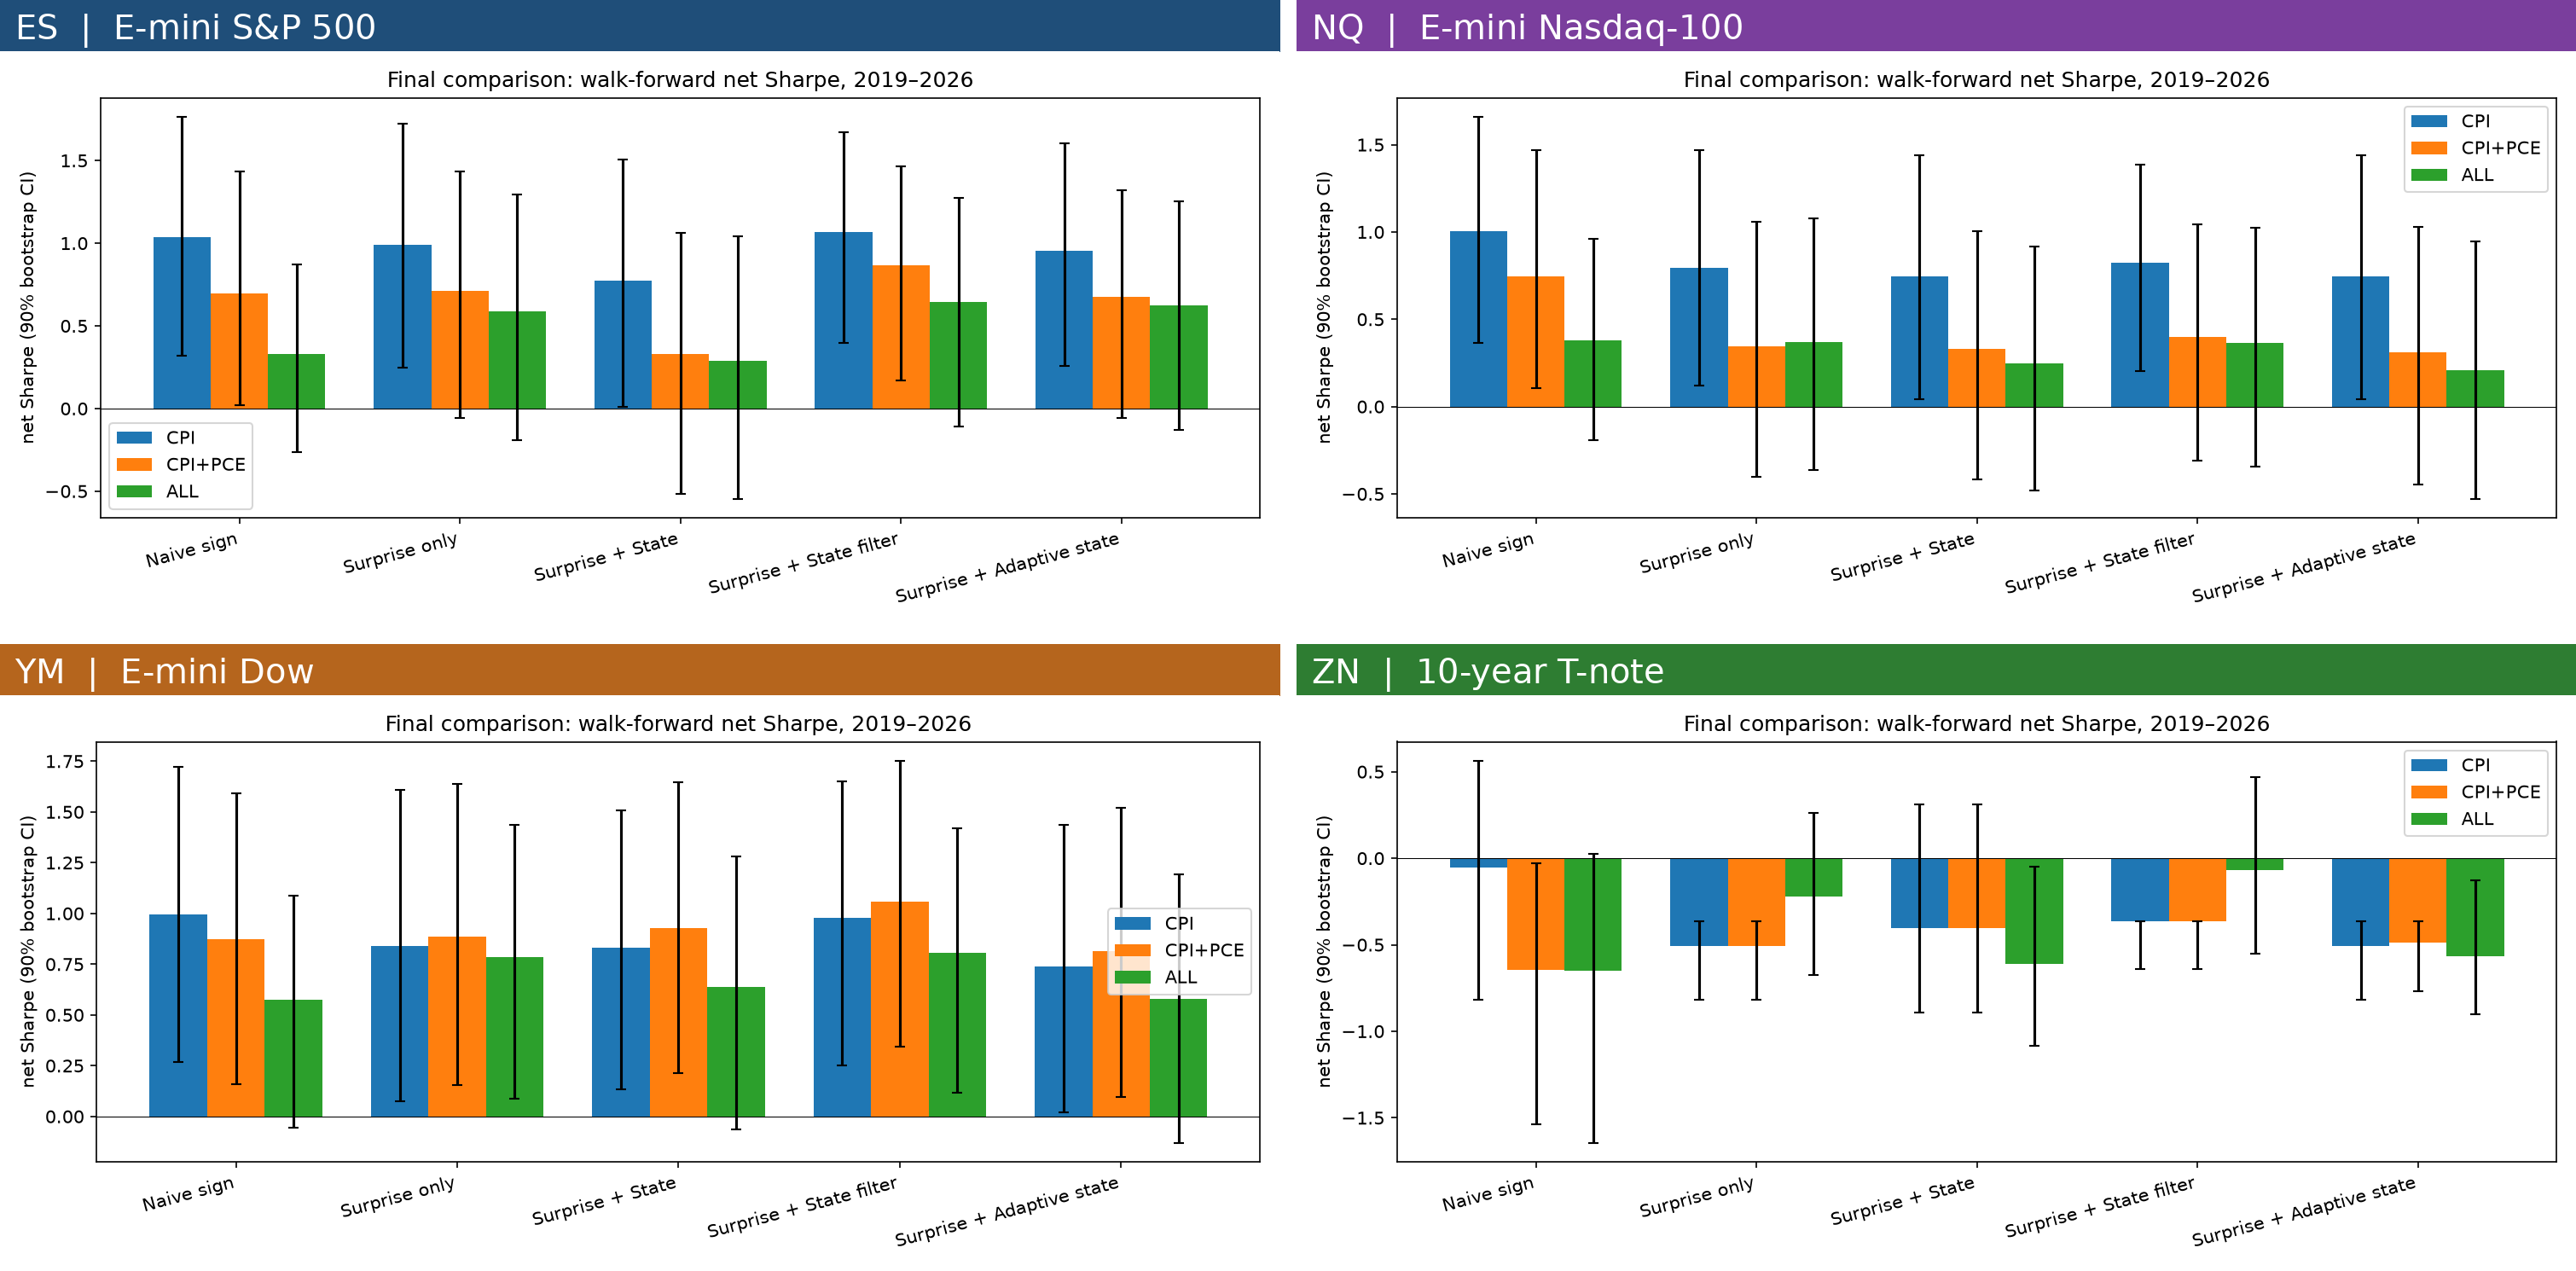
\includegraphics[width=0.8\linewidth]{fig19_final_sharpe_4markets}
  \caption{Net Sharpe ratio of the CPI strategies (naive, surprise model and three state-conditioned
  models) in three release universes (CPI; CPI + PCE; CPI + PCE + NFP), \ES, \NQ, \YM\ and \ZN,
  2019--2026, at 2 ticks + \$4.50.}
\end{figure}

No state-conditioned model significantly beats the surprise-only model in any market: the change
in Sharpe ratio ranges from $-0.21$ to $+0.08$ in \ES, from $-0.05$ to $+0.03$ in \NQ\ and from $-0.20$ to $+0.17$ in \YM, where no difference is
significant (smallest bootstrap $p=0.23$). Adding PCE
and NFP to CPI dilutes the signal in \ES\ (surprise-only Sharpe 0.99, 0.71 and 0.59) but much less
in \YM\ (0.84, 0.89 and 0.78).

\section{Reproducibility map}
\begin{table}[htbp]
  \centering\small
  \caption{Programs that produce each exhibit (repository \url{https://github.com/jack-duncan/blackrock-intraday}).}
  \begin{tabular}{ll}
    \toprule
    Exhibit & Program \\
    \midrule
    Figures 1--3, Table 3 & \texttt{Reza/notebooks/02\_event\_response\_analysis}, \texttt{02b} \\
    Figure 4 & \texttt{Reza/notebooks/03\_state\_conditioning}, \texttt{03b} \\
    Sections V.A--B and VII, Figures 6, 9--10 & \texttt{Reza/notebooks/04}--\texttt{06} and \texttt{b} versions \\
    Table 5 & \texttt{Reza/notebooks/08\_team\_comparison\_equal\_costs} \\
    Figure 7 & \texttt{combined/surprise\_dtw\_book} \\
    Tables 4 and 6, Figure 8 & \texttt{combined/team\_book} \\
    DTW construction grids & \texttt{combined\_modified\_hoshea}, \texttt{hoshea\_zeng/es\_only} \\
    \bottomrule
  \end{tabular}
\end{table}

\end{document}
